\subsection{Model fitting}
\label{subsec:fitting}
We employed a Markov Chain Monte Carlo (MCMC) script to fit the coefficients of a polynomial model for $r(\mathcal{M}_c)$. The MCMC uses the smoothing prior as defined in \S\ref{subsec:likelihood}. We performed a least square fit first in order to obtain the initial guess for the coefficients of the model.

The model we used is a polynomial of degree 4. Because of the smoothing function, using higher order does not change the shape of the fit in a significant way. The MCMC best fit can be seen in Figure \ref{fig:line_MCMC}. The MCMC walkers and triangle plot are in Figures \ref{fig:MCMC_time} and \ref{fig:MCMC_triangle}.

Best fit model is:
\begin{equation}
\label{MCMC_best_fit}
\log r(\mathcal{M}_c) = -7.3107 (\log\mathcal{M}_c)^4 + 5.0419 (\log\mathcal{M}_c)^3 + 1.0809 (\log\mathcal{M}_c)^2 + 14.2431 \log\mathcal{M}_c - 4.0667
\end{equation}

\begin{figure}[ht]
  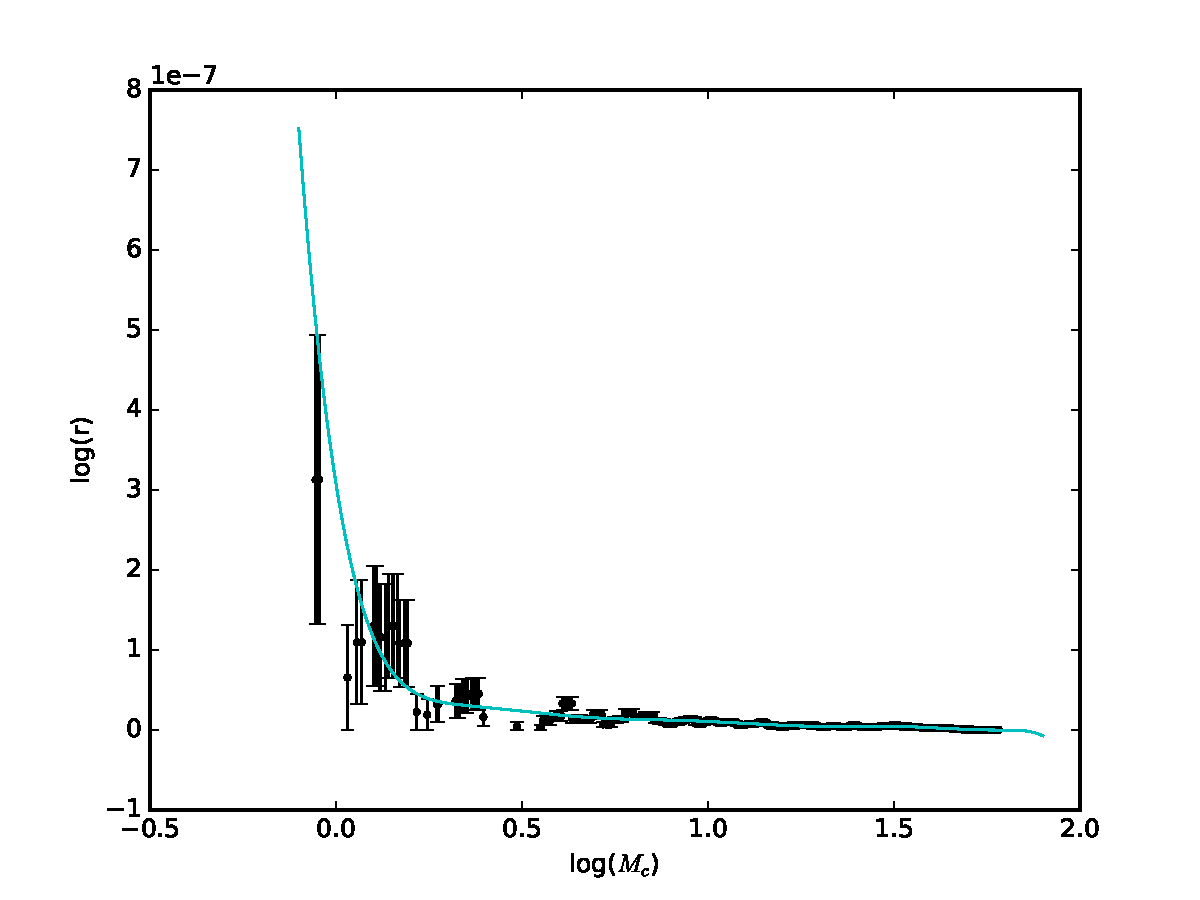
\includegraphics[width=\columnwidth]{img/line-MCMC.pdf}
  \caption{100 randomly chosen fits from the MCMC.}
  \label{fig:line_MCMC}
\end{figure}

\begin{figure}[ht]
  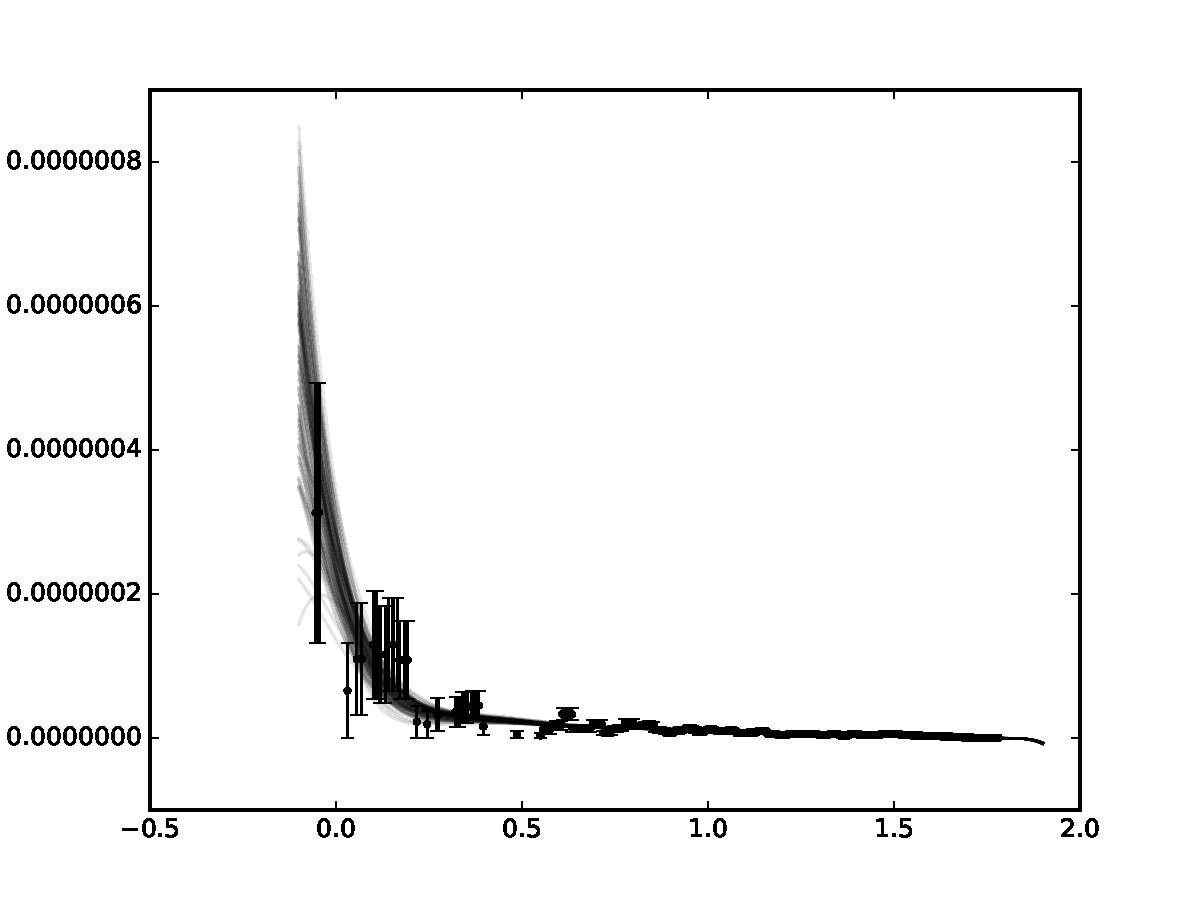
\includegraphics[width=\columnwidth]{img/line-mcmc_err.pdf}
  \caption{The cyan line is an example of a fit from MCMC.}
  \label{fig:line_MCMC}
\end{figure}


\begin{figure}[ht]
  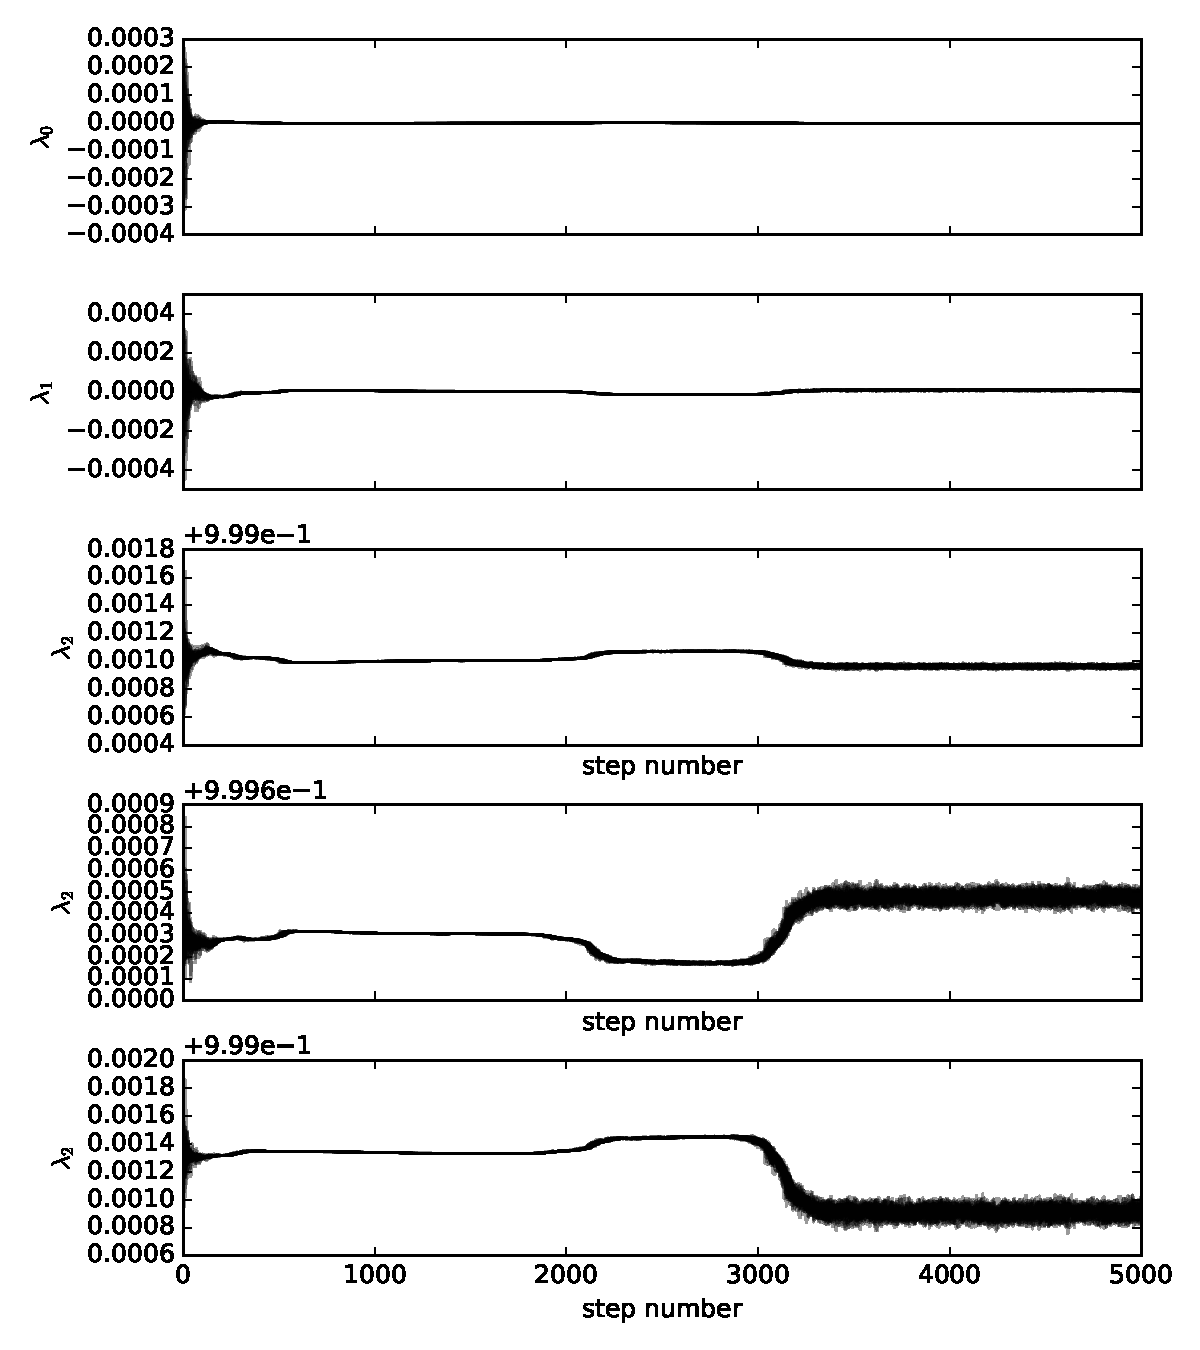
\includegraphics[width=\columnwidth]{img/line-time.pdf}
  \caption{MCMC workers converging.}
  \label{fig:MCMC_time}
\end{figure}

\begin{figure}[ht]
  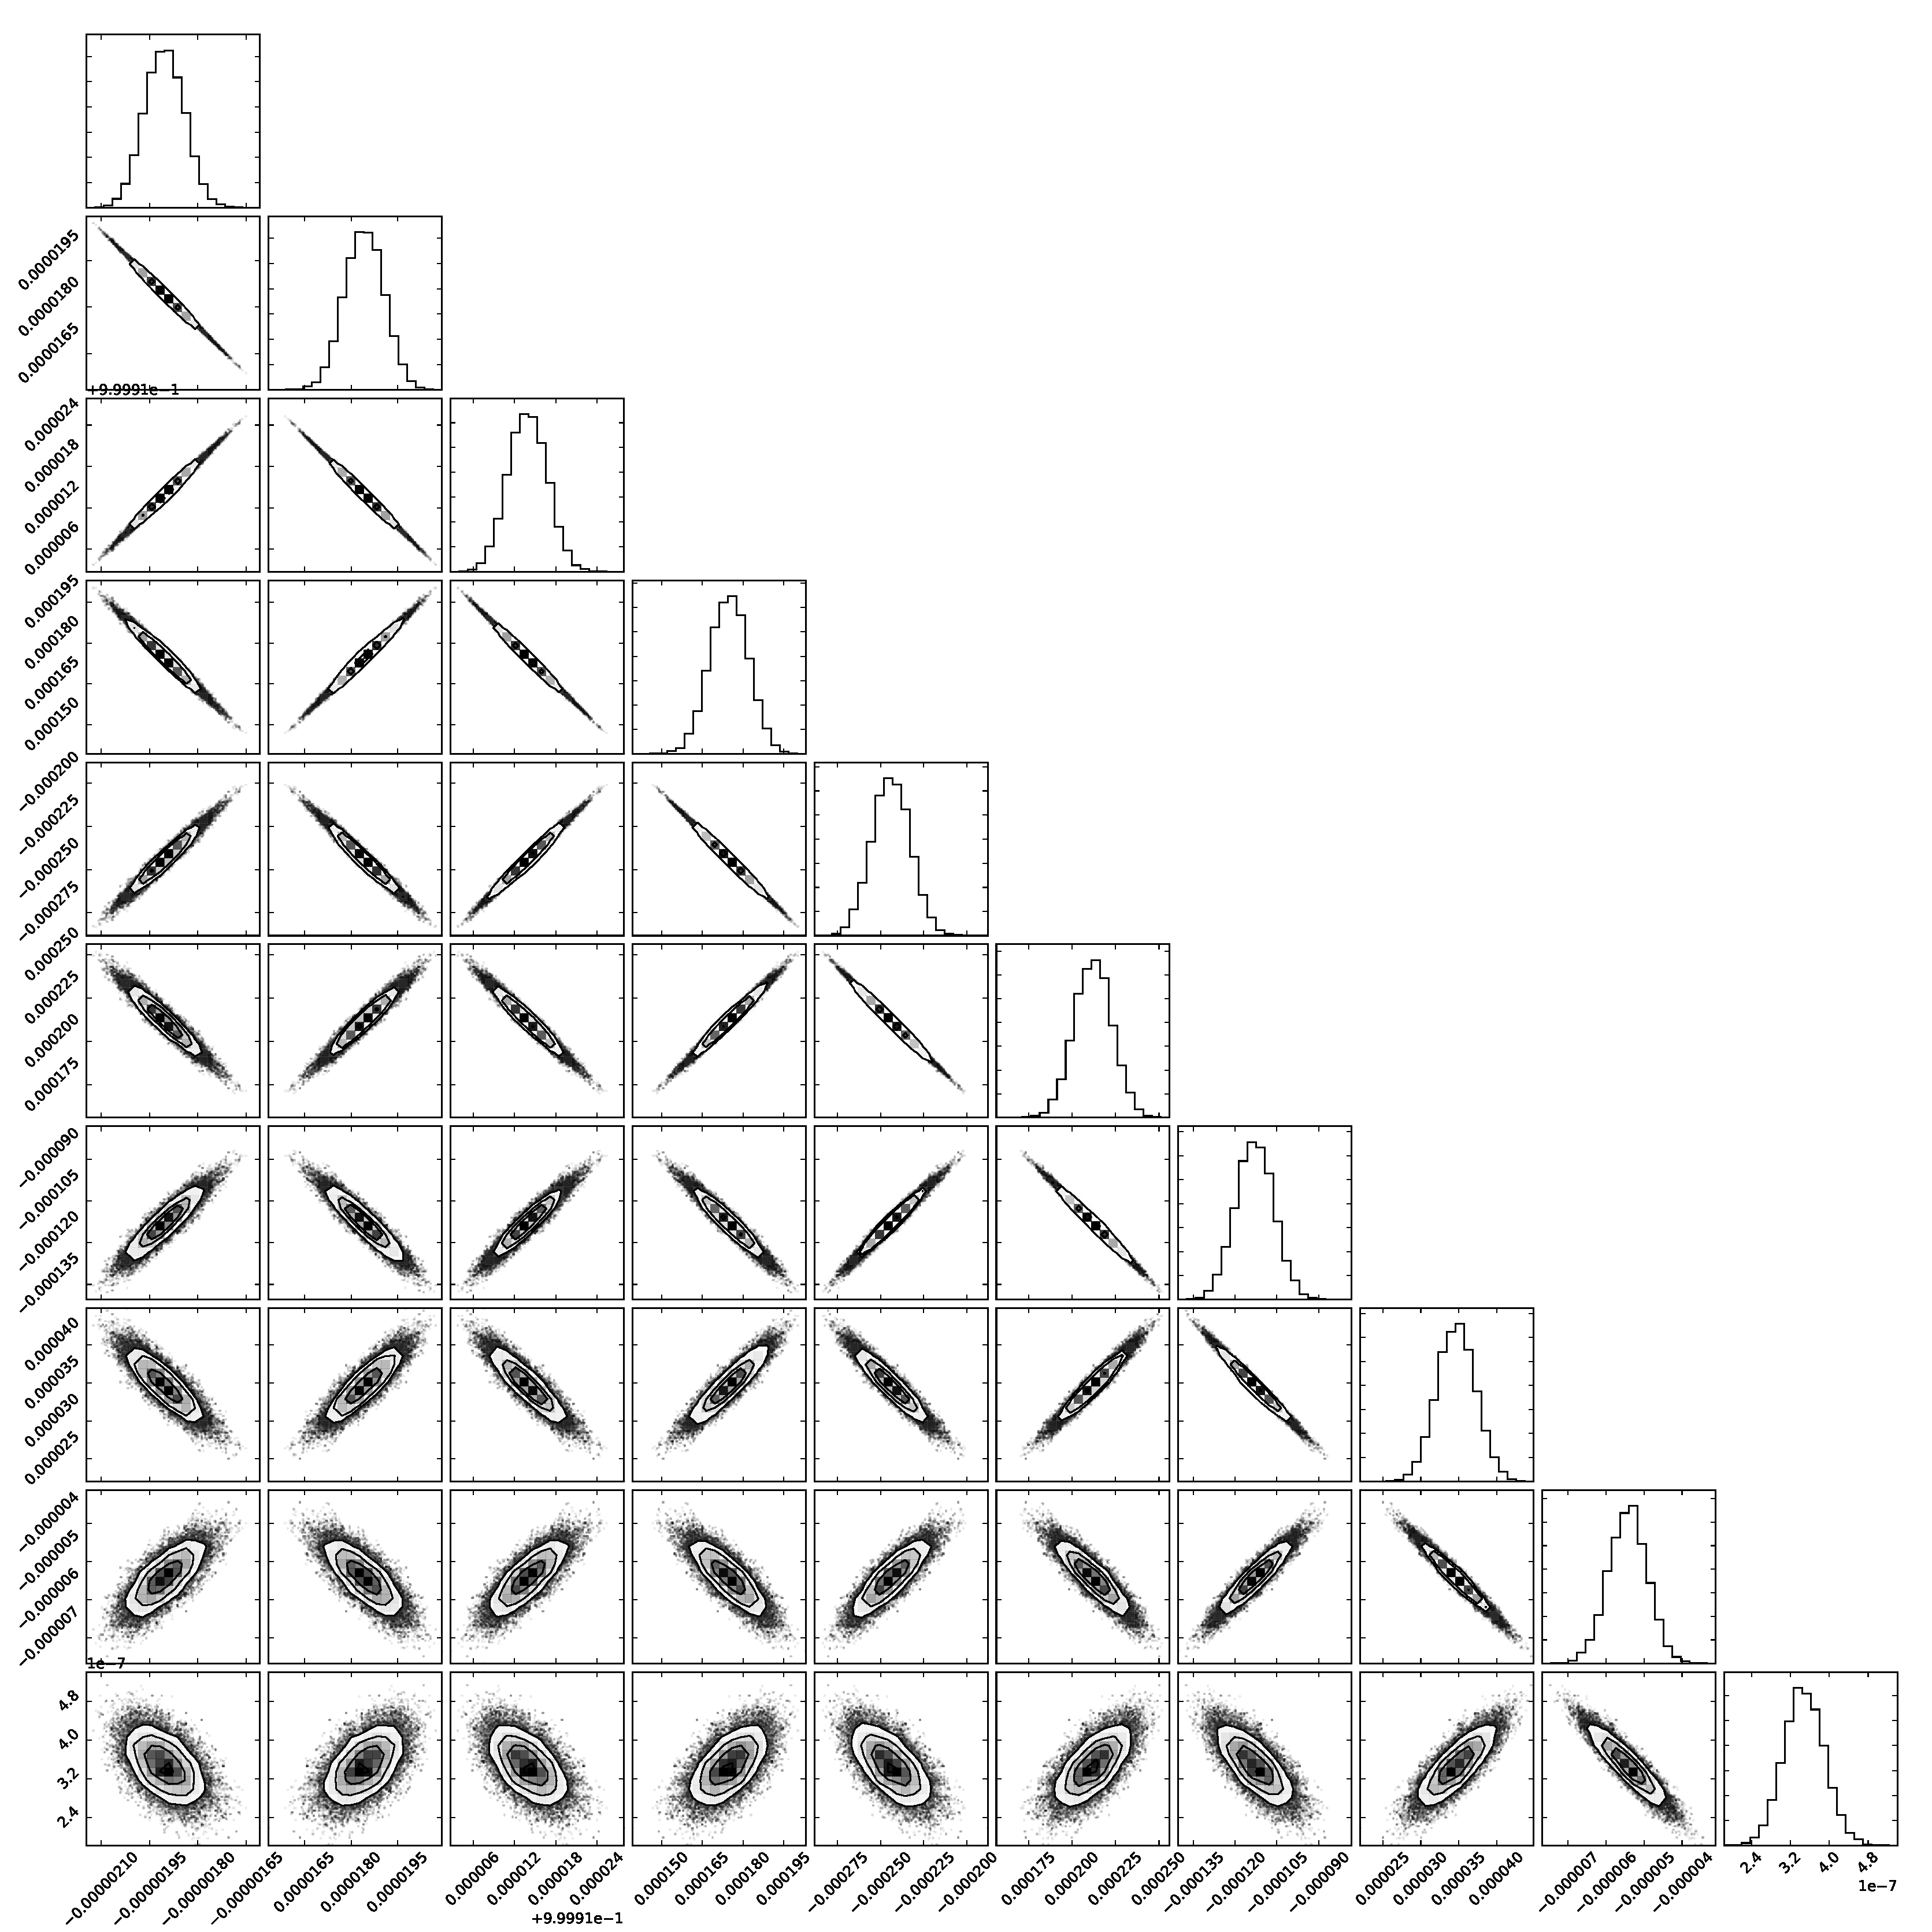
\includegraphics[width=\columnwidth]{img/line-triangle.pdf}
  \caption{Corner plot of MCMC fit coefficients.}
  \label{fig:MCMC_triangle}
\end{figure}

